\documentclass[12pt,preprint]{aastex}
%\documentclass{emulateapj}
%\documentclass{mn2e}
%\bibliographystyle{mn2e}
%\usepackage{Times}
%\usepackage{subfigure}
%\usepackage{epsfig}
%\usepackage{amsmath}
%\usepackage{graphicx}
%\newcommand{\tmin}{{T_{\rm min}}}
%\newcommand{\msun}{M_{\odot}}
%\newcommand{\ion}[2]{#1$\;${\small\rmfamily{#2}}\relax}% regular \ion generates error



%\title[Cluster versus Redshift]{Cluster vs Redshift}
%\author[S. Tonnesen and R. Cen]{Stephanie Tonnesen$^{1}$\thanks{E-mail:  stonnes@astro.princeton.edu (ST);  cen@astro.princeton.edu (RC)} and Renyue Cen$^{1}$\\
%$^{1}$Department of Astrophysics, Princeton University, Peyton Hall, Princeton, NJ, 08544\\
%}
\begin{document}
\section{Building a Gas-Rich Dwarf Satellite}

I am loosely basing my model on IC1613 because Josh Simon has HI rotation curve data for that galaxy and it isn't ridiculously teensy.  According to Mateo (1998), distance is 700 kpc, although this may be a bit low (750 kpc in later papers?).\\

\subsection{Dark Matter Potential}

\noindent From Mateo ARAA (1998) tables, the central mass density is:\\
\indent $\rho$$_{o}$ $=$ 0.035 M$_{\odot}$ pc$^{-2}$ = 2.37e-24 g cm$^{-3}$\\


\noindent Using the Burkert (1995) DM profile, this gives me everything else about the halo:\\
\indent r$_{o}$ = 1.5 kpc\\
\indent M$_{o}$ = 1.84e8 M$_{\odot}$ (The mass contained within r$_{o}$)\\
\indent v$_{c,max}$ = 30 km/s\\

This is not too bad in comparison to other data:  Lake \& Skillman (1989) observe a maximum rotation velocity of 25 km/s, but this may be a lower limit (according to Skillman et al. 2014).  \\

However, the inner rotation curive in Lake \& Skillman (1989) increases more slowly than anything with the Burkert (1995) DM profile.  The fit in the central region is better with a lower mass halo (but still not great), so I have gone with:\\

\indent r$_{o}$ = 1.144 kpc\\
\indent $\rho$$_{o}$ $=$ 2.8188e-24 g cm$^{-3}$\\
\indent M$_{o}$ = 1e8 M$_{\odot}$ (The mass contained within r$_{o}$)\\
\indent v$_{c,max}$ = 25 km/s\\


\subsection{Stellar Potential}

Stellar mass 10$^8$ M$_{\odot}$ (McConnachie 2012, via Skillman et al. 2014).  \\
From Mateo (1998), r$_{exp}$ = 5.4' = 1.099 kpc\\
According to McConnachie \& Irwin (2006), the Plummer profile b $\sim$ 1.68r$_e$ of the exponential profile, so b = 1.85 kpc.  I am using a Plummer-Kuzmin disk (Miyamoto \& Nagai 1975; MN75), so also need to choose an a. According to Mateo (1998) at large radius the ellipticity is 0.24, so based on eyeing figures in MN75 I choose a = 2 kpc.  Changing these values does very little to the rotation curve.\\

I choose to use no bulge (actually a 1 solar mass bulge), but that can change!\\

%Lake \& Skillman (1989) find an outer axis ratio of 0.79, which corresponds to an inclination of 38 degrees for a thin disk. 
 
\subsection{Gas Disk}

How flattened is the gas disk--does the major axis = minor axis?  My code fails at a/b $<$ 3, so that is the limit on sphericity.\\

From Mateo (1998) M$_{HI}$= 5.4e7 M$_{\odot}$.  In order to get N(H) at R = 0 of $\sim$3.2e20 cm$^{-2}$, I need an a (R scale height) of 2.8 kpc and a b (z scale height) of 1 kpc.   

\section{Surrounding IGM/CGM}

Right now I just need a low-density guess for static surrounding gas.  I may have gone a bit too high-density, high-pressure.  \\
\indent $\rho$= 1e-28 g cm$^{-3}$\\
\indent T = 10$^6$ K\\

Looks like from Diemer \& Kravtsov (2014) I should be more like 4e-29 for the density, so will have to make that change.  I think having the surrounding gas a little high is not too bad, because it will lower the mach number of the shock for a constant strong wind....

\begin{figure}
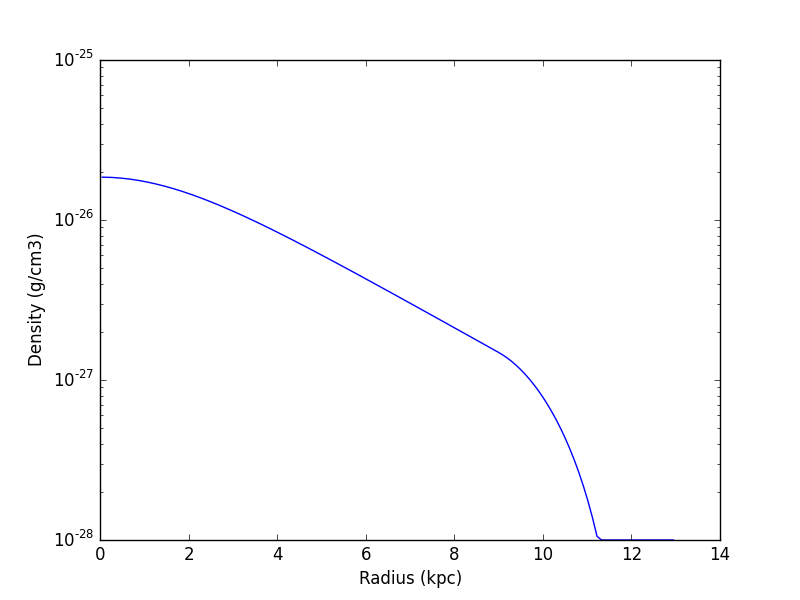
\includegraphics[scale=0.5]{dwarf_density_profile.png}\\
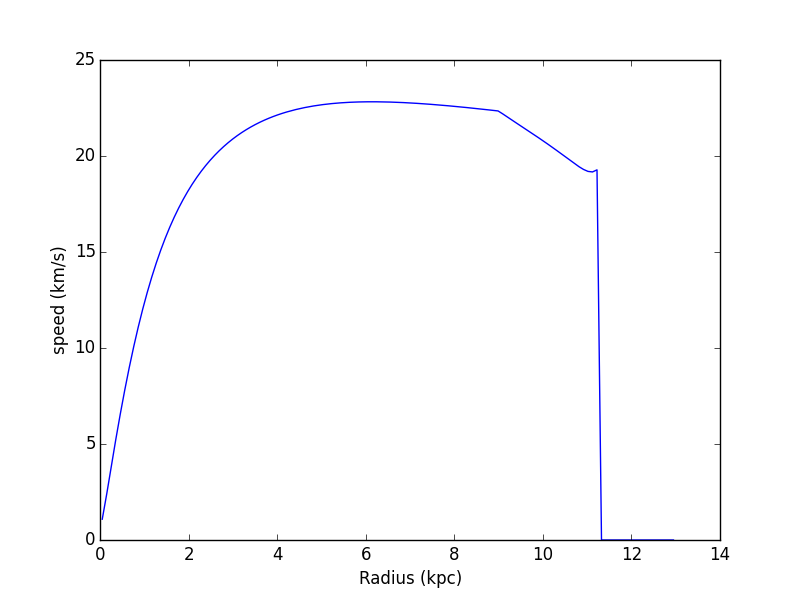
\includegraphics[scale=0.5]{dwarf_rotation_profile.png}\\
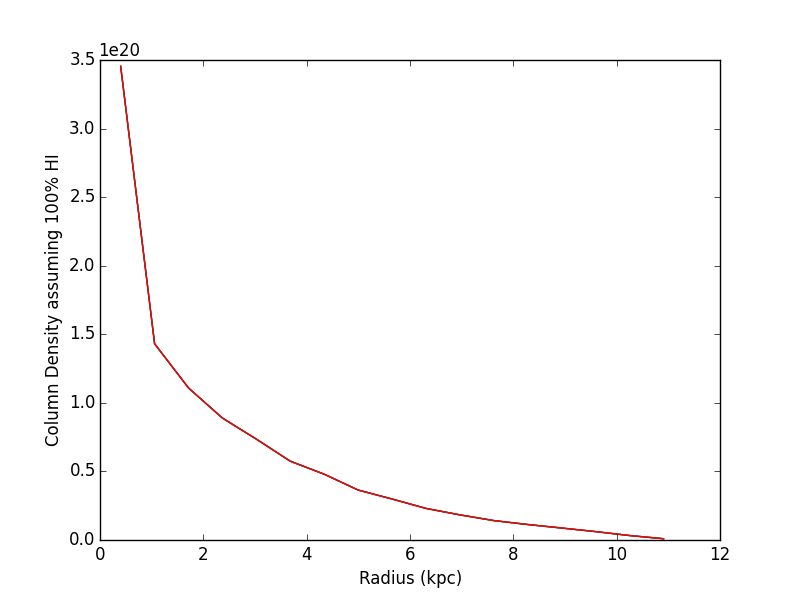
\includegraphics[scale=0.5]{dwarf_coldens_profile.png}
\end{figure}





\section{Random Notes}

A larger b$_{gas}$ leads to a slower rotation curve, but a higher maximum gas pressure in the disk (read:  higher temp!).  

A smaller a$_{gas}$ leads to a slower rotation curve--I get the impression that a/b $<$ 3 will crash, but otherwise you want it as small as possible.  

A larger a$_{stars}$ leads to a slower rotation curve--but going from 2 kpc to 8 kpc changed the peak from 0.008779 to 0.008565, so not a huge effect.  

A larger b$_{stars}$ leads to a slower rotation curve--but from .4625 kpc to 7.4 kpc the curve changed from 0.008812 to 0.008601, so not a big change.  

\end{document}